\section{Basic concepts}

\begin{frame}{Floors and Ceilings}
\begin{definition}
    \begin{itemize}
        \item $\lfloor x \rfloor$ = the greatest integer less 
        than or equal to $x$. 
        \item $\lceil x \rceil$ = the least integer greater 
        than or equal to $x$. 
    \end{itemize}
\end{definition}

    \begin{figure}
        \centering
        
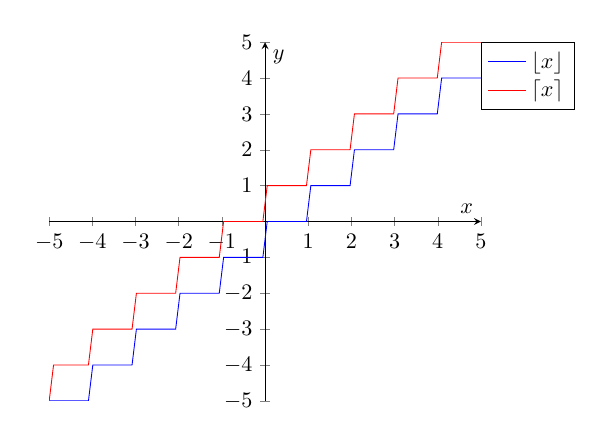
\begin{tikzpicture}[scale=0.8]
    \begin{axis}[
      xlabel=$x$,
      ylabel=$y$,
      axis lines=middle,
      ymin=-5, ymax=5,
      xmin=-5, xmax=5,
      xtick={-5,-4,-3,-2,-1,0,1,2,3,4,5},
      ytick={-5,-4,-3,-2,-1,0,1,2,3,4,5},
      legend pos=north west,
      legend style={at={(1,1)},anchor=north west}
    ]
    
    % Floor function
    \addplot[color=blue,domain=-5:5,samples=100] {floor(x)};
    \addlegendentry{$\lfloor x \rfloor$}
    
    % Ceiling function
    \addplot[color=red,domain=-5:5,samples=100] {ceil(x)};
    \addlegendentry{$\lceil x \rceil$}
    
    \end{axis}
  \end{tikzpicture}
        \caption{Floor and ceiling}
    \end{figure}
\end{frame}

\begin{frame}{Basic Properties}
    \begin{itemize}
        \item Inequality: $x-1<\lfloor x\rfloor \leq x \leq \lceil x \rceil<x+1$. 
        \item Negation: $\lceil -x \rceil = -\lfloor x \rfloor$, $\lfloor -x \rfloor = -\lceil x\rceil$. 
        \item \textbf{Convert}: 
        \begin{itemize}
            \item $\lfloor x \rfloor = n \iff \visible<2->{ n\leq x < n+1} $ (with respect to $x$);
            \item $\lfloor x \rfloor = n \iff \visible<2->{ x-1\leq n < x}$ (with respect to $n$);
            \item $\lceil x \rceil = n \iff \visible<2->{ n-1 < x \leq n} $ (with respect to $x$);
            \item $\lceil x \rceil = n \iff \visible<2->{ x\leq n < x+1}$ (with respect to $n$);
        \end{itemize}
        \item Moving integers: For integer $n$, $\lfloor x+n \rfloor=\lfloor x \rfloor+n$.
    \end{itemize}
    
\end{frame}

\begin{frame}{Example. An identity}
 \begin{example}
     Prove that $\lfloor \sqrt{\lfloor x \rfloor} \rfloor = \lfloor \sqrt{x} \rfloor$.
 \end{example}
    
    \pause
    \begin{itemize}
        \item Let $m=\lfloor \sqrt{\lfloor x \rfloor} \rfloor$. What is the range of $m$? 
        \item $m\leq \sqrt{\lfloor x \rfloor} < m+1$. 
        \item Squaring to get the answer. 
    \end{itemize}
    
\end{frame}

\begin{frame}{Example. Switching counting number}
\begin{example}
    Let $f(x)$ be any cont. mono. increasing func. with prop. that 
    $f(x) = \text{integer } \implies x=\text{integer}$, prove that 
    $\lfloor f(x) \rfloor = f(\lfloor x \rfloor)$, same as the ceiling. 
\end{example}

\pause 
\begin{itemize}
    \item If $x=\lfloor x \rfloor$, trivial. 
    \item Otherwise $x>\lfloor x \rfloor \implies f(x)>f(\lfloor x \rfloor)$. What about $f(\lfloor x \rfloor)$ and $\lfloor f( x )\rfloor$? 
    \begin{itemize}
        \item Assume this is true: $f(\lfloor x \rfloor)<\lfloor f( x )\rfloor$, continuous, 
        \item must be a number $y$ s.t. $x\leq y < \lceil x \rceil$ and $f(y)=\lceil f(x) \rceil$. By the special property of $x$
        \item $y$ integer, no number between $x\leq y < \lceil x \rceil$, hence they are equal. 
    \end{itemize}

    Same problem: cont. mono. decreasing, what's that?
\end{itemize}
\end{frame}

\begin{frame}{Counting the Integer Points}
    Count the integer points on a number line. 
    \begin{itemize}
        \item if $a, b\in \mathbb Z$, integer point in $[a, b]$ is 
        $b-a+1$.
        \item More general case
        \begin{itemize}
            \item $[\alpha, \beta] \qquad \visible<2->{\flr{\beta}-\cil{\alpha}+1}$
            \item $(\alpha, \beta] \qquad \visible<2->{\flr{\beta}-\flr{\alpha}}$
            \item $[\alpha, \beta) \qquad \visible<2->{\flr{\beta}-\cil{\alpha}}$
            \item $(\alpha, \beta) \qquad \visible<2->{\cil{\beta}-\flr{\alpha}-1}$
        \end{itemize}
    \end{itemize}

    Helpful when handling summations by counting. 
\end{frame}

\begin{frame}{Example. Computing a sum}

\begin{example}
     Compute 
    $$
    W=\sum_{i=1}^{1000} [\cil{\sqrt[3]{n}} | n]
    $$ 
\end{example}

\pause 

\begin{itemize}
    \item Make a new one name for $k=\sqrt[3]n$, getting $k\mid n, 1\leq n\leq 1000$. 
    \item The range for $k$ is $k\leq \sqrt[3]{n}<k+1$
    \item $k|n$ means that there is a $m$ so that $n=km$. 
    \item then becomes $1+\sum_{k,m} [k^3\leq km \leq (k+1)^3][1\leq k<10]$. 
\end{itemize}

\end{frame}
    
\begin{frame}{Example cont'd. Computing a sum}

\begin{example}
    Compute 
    $$
    W=\sum_{i=1}^{K} [\cil{\sqrt[3]{n}} | n], K\in \Z. 
    $$ 
\end{example}


\pause 

\begin{itemize}
    \item We should care about $\sum_m[k^3\leq Km\leq N]$.
    \item this part become $\sum_m [m\in [k^2..N/K]]$. 
    \item the estimation will be $3/2N^{2/3}+O(N^{1/3})$. 
\end{itemize}
    
\end{frame}

\begin{frame}{Example. The Spectra Example}

\begin{example}
    The \underline{spectrum} of a real number $\alpha$ to be an 
    infinite multiset of integers. That is
    $$
    \text{Spec}(\alpha) = \{\cil{\alpha}, \cil{2\alpha}, \cdots\}
    $$
    We can prove that (1) no two spectrum are equal; (2) $\text{Spec}(2)\cup \text{Spec}(2+\sqrt{2}) = \Z$. 
\end{example}

\pause 

\begin{itemize}
    \item We define $N(\alpha, n)=\sum _{k>0}[\flr{k\alpha}\leq n]$.
    \item which is $\cil{(n+1)/\alpha}-1$. 
    \item proving $\cil{n+1/\sqrt2}-1+\cil{n+1/2+\sqrt2}-1=n$. 

\end{itemize}

This equality will be helpful: 
$$
a\leq b \implies a<b-1 \text{ for floors and ceiling func.}
$$

\end{frame}




